
\chapter{Constructing a Reference Pathtracer}
\label{chap:pathtracing}

\section{Solving the Rendering Equation}

As always in rendering, we are interested in solving the rendering equation, which describes how light interacts with surfaces in a scene and was first introduced by \textcite{kajiya1986}.
The rendering equation is given by:
\begin{equation}
\label{eq:rendering_equation}
    L_o(\vec{x}, \wo) = L_e(\vec{x}, \wo) + \int_{\Omega} f(\wi, \vec{x}, \wo) L_i(\vec{x}, \wi) \cos\theta_i \diff\wi
\end{equation}
where $L_o$ is the outgoing radiance, $L_e$ is the emitted radiance, $f$ is the bidirectional scattering distribution function (BSDF), $L_i$ is the incoming radiance from direction $\omega_i$, and $\theta_i$ is the incident angle, which is the angle between the incoming light direction $\omega_i$ and the surface normal at $\vec{x}$.

\section{Monte Carlo Integration}

The rendering equation is an infinite recursive integral over all possible light paths, for which no closed-form solution exists in general.
Hence, to solve it we need to resort to numerical integration strategies.
Deterministic integration methods suffer from the curse of dimensionality as the rendering equation is notoriously high dimensional.
Thus, we utilize probabilistic approaches to solve it.
We will use Monte Carlo integration, which was originally developed by \textcite{metropolis1949} as part of the Manhattan Project and first introduced to rendering by \textcite{kajiya1986}.
The idea is, to compute the integral using random samples drawn from a probability distribution, which ideally is chosen as proportional to the integrand as possible.

Applying this to the rendering equation, we can formulate an estimator for the outgoing radiance $L_o$:
\begin{equation}
    \estimator{I_\mathrm{MC}} = L_e(\vec{x}, \wo) + \frac{1}{N} \sum_{i=1}^{N} \frac{f(\vec{\hat{\omega}}_i, \vec{x}, \wo) \cos(\hat{\theta}_i)}{p(\vec{\hat{\omega}}_i \mid \wo)} L_i(\vec{x}, \vec{\hat{\omega}}_i), \quad \vec{\hat{\omega}}_i \sim p(\vec{\hat{\omega}}_i \mid \wo)
\end{equation}

This is an unbiased estimator for the rendering equation, as can be easily shown:
\begin{equation}
    \begin{aligned}
        \expectation{\estimator{I_\mathrm{MC}}}
        &= L_e(\vec{x}, \wo) + \cancel{\frac{1}{N}} \cancel{\sum_{i=1}^{N}} \expectationvar{\vec{\hat{\omega}}_i \sim p(\vec{\hat{\omega}}_i \mid \wo)}{\frac{f(\vec{\hat{\omega}}_i, \vec{x}, \wo) \cos(\hat{\theta}_i)}{p(\vec{\hat{\omega}}_i \mid \wo)} L_i(\vec{x}, \vec{\hat{\omega}}_i)} \\
        &= L_e(\vec{x}, \wo) + \int_{\Omega} \frac{f(\vec{\hat{\omega}}_i, \vec{x}, \wo) \cos(\hat{\theta}_i) \cancel{p(\vec{\hat{\omega}}_i \mid \wo)}}{\cancel{p(\vec{\hat{\omega}}_i \mid \wo)}} L_i(\vec{x}, \vec{\hat{\omega}}_i) \diff\wi \\
        &= L_o(\vec{x}, \wo)
    \end{aligned}
\end{equation}
Hence, by the law of large numbers this estimator converges to the true solution to the rendering equation for $N \to \infty$.

To handle the infinite recursion without introducing bias, I use Russian Roulette Termination as motivated by \textcite{veach1997}, which probabilistically terminates the recursion based on the contribution of the current path segment:
\begin{equation}
\label{eq:rr}
    \estimator{I_\mathrm{RR}} =
    \begin{cases}
        \frac{\estimator{I_\mathrm{MC}}}{p_\mathrm{continue}} & \text{with probability } p_\mathrm{continue} \\
        0 & \text{with probability } 1 - p_\mathrm{continue}
    \end{cases}
\end{equation}
The probability terms cancel out, thus this modification to the estimator does not introduce bias.
I choose $p_\mathrm{continue}$ proportional to the relative luminance $Y$ \parencite{kirkpatrick2025} of the contribution of the current path segment, which measures the perceived linear brightness of that sample:
\begin{equation}
\label{eq:luminance}
    Y(\vec{c}) = 0.2126 \cdot c_r + 0.7152 \cdot c_g + 0.0722 \cdot c_b
\end{equation}

% With this and by introducing a visibility term $V$, we can estimate the collected radiance along a complete path in an unbiased manner:
% \begin{equation}
%     L_o(\vec{x^0}, \wo^0) = \frac{1}{N} \sum_{i=1}^{N} L_e(\vec{x^1}, \wo^1) + \frac{f(\wi^1, \wo^1) \cos(\theta_i^1)}{p_\mathrm{continue} p(\wi^1)} \cdot \left( L_e(\vec{x^2}, \wo^2) + \frac{f(\wi^2, \wo^2) \cos(\theta_i^2)}{p_\mathrm{continue} p(\wi^2)} \cdot \left(\cdots\right) \right)
% \end{equation}

\section{Randomized Quasi-Monte Carlo Integration}

To improve the convergence of the Monte Carlo integration, low-discrepancy sequences can be used instead of purely random samples.
Low-discrepancy sequence are designed to fill the integration domain more uniformly than random samples, which can lead to a lower variance in the estimator.
This approach is called Quasi-Monte Carlo integration and was first introduced to rendering by \textcite{heinrich1994a}.
\textcite{keller1996a} later showed faster convergence of Quasi-Monte Carlo integration compared to random Monte Carlo integration in exemplary path tracing scenarios.

Carefully introducing randomness to the low-discrepancy sequence can help to improve convergence further and mitigate visible artifacts caused by the deterministic nature of such sequences.
This is known as Randomized Quasi-Monte Carlo integration and was first introduced by \textcite{owen1995}.
For a practical application to path tracing see for example \textcite{burley2020}.

I use the scrambled Sobol' sequence from cuRAND \parencite{nvidiacorporation2024} which is based on the work of \textcite{owen2008}.
Furthermore, I employ the same technique as the \textcite{blenderfoundation} and only precompute a single Sobol' sequence for the entire scene, which is then decorrelated between pixels using constant random per-pixel shifts modulo 1, also known as Cranley-Patterson rotations \parencite{cranley1976}.
The Sobol' sequence is regularly recomputed in batches on the GPU to allow for unlimited progressive rendering, the per pixel shifts are only recomputed on frame buffer resize, which makes this technique relatively lightweight.

\section{Principled BSDF}

As a material model we will use a simplified physically based model, which is inspired by the Disney principled BSDF \parencite{burley2012} and conformant with the glTF PBR specification \parencite{thekhronosr3dformatsworkinggroup2021}.
The BSDF will be restricted to the diffuse, specular and transmission components, as they can already cover a wide range of interesting materials and suffice to showcase the strengths and weaknesses of the subsequent techniques.

The BSDF is split into two parts: If the light direction $\wi$ and the view direction $\wo$ lie in the same hemisphere, the BSDF is composed of a diffuse and a specular lobe, otherwise it only consists of a transmission lobe:
\begin{equation}
    f(\wi, \vec{x}, \wo) =
    \begin{cases}
        f_s(\wi, \vec{x}, \wo) + f_d(\wi, \vec{x}, \wo) & \text{if } \NdotL \cdot \NdotV > 0 \\
        f_t(\wi, \vec{x}, \wo) & \text{otherwise}
    \end{cases}
\end{equation}

\begin{figure}[htb!]
\begin{subfigure}{.5\textwidth}
    \centering
    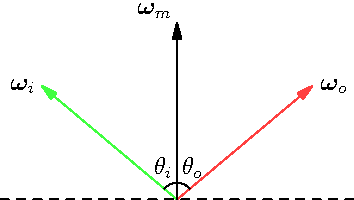
\includegraphics{asy/wm_reflect.pdf}
    \caption{Reflection}
    \label{fig:wm_reflect}
\end{subfigure}%
\begin{subfigure}{.5\textwidth}
    \centering
    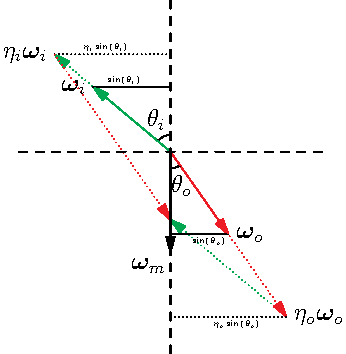
\includegraphics{asy/wm_refract.pdf}
    \caption{Refraction}
    \label{fig:wm_refract}
\end{subfigure}
\caption{
\textbf{(a)} For the reflective case, the halfvector $\wm$ lies simply in the middle of the incident and outgoing direction.
\textbf{(b)} We can obtain the halfvector $\wm$ for the refractive case by summing $\eta_i \wi$ and $\eta_o \wo$, where $\eta_i$ and $\eta_o$ are the indices of refraction of the incident and outgoing medium, respectively. The orthogonal components of $\wi$ and $\wo$ are simply the sine, so by weighting and summing them they cancel out according to Snell's law.
}
\end{figure}

For the specular component, we will use the Torrance-Sparrow/Cook-Torrance microfacet model \parencite{torrance1967, cook1982} with the corrected normalization factor from \textcite{walter2007}:
\begin{equation}
    f_s(\wi, \vec{x}, \wo) = \frac{D(\NdotH) G(\n, \wi, \wo) F(\LdotH)}{4 \NdotL \NdotV}
\end{equation}
where $D$ is the isotropic Trowbridge-Reitz normal distribution function (NDF) originally defined by \textcite{trowbridge1975} and later rediscovered by \textcite{walter2007}:
\begin{equation}
    D(\NdotH) = \frac{\alpha^2}{\pi (\alpha^2 \cos^2 \theta_m + \sin^2 \theta_m)^2}
\end{equation}
Here, $\alpha$ is the width of the microfacet distribution, which is related to the roughness of the surface.
$\wm$ is the normal of an ideally reflecting microfacet (see \cref{fig:wm_reflect}):
\begin{equation}
    \wm = \frac{\wi + \wo}{\|\wi + \wo\|}
\end{equation}

$G$ is the corresponding geometric attenuation term, for which I use the Smith shadowing-masking function \parencite{smith1967}, derived for the Trowbridge-Reitz NDF by \textcite{walter2007}:
\begin{equation}
    \begin{aligned}
    G(\n, \wi, \wo) &= \frac{1}{1 + \Lambda(\NdotL) + \Lambda(\NdotV)}\\
    \quad \text{with } \quad
    \Lambda(\NdotX) &= \frac{1}{2} \left( \sqrt{1 + \alpha^2 \mathrm{tan}^2 \theta} - 1 \right)
    \end{aligned}
\end{equation}

For the Fresnel term $F$, I use the Schlick approximation \parencite{schlick1994}:
\begin{equation}
    F(\LdotH) = F_0 + (1 - F_0) (1 - \LdotH)^5
\end{equation}

In the case of transmission, the normal of an ideally refracting microfacet is given by (see \cref{fig:wm_refract}):
\begin{equation}
    \wm = \pm\frac{\eta_i \wi + \eta_o \wo}{\|\eta_i \wi + \eta_o \wo\|} = \pm\frac{\eta \wi + \wo}{\|\eta \wi + \wo\|}
\end{equation}
where $\eta = \frac{\eta_i}{\eta_o}$ is the relative index of refraction (IOR).
The transmission component is then the following, as derived by \textcite{walter2007}:
\begin{equation}
    f_t(\wi, \vec{x}, \wo) = \rho_t \frac{D(\NdotH) G(\n, \wi, \wo) (1 - F(\LdotH))}{(\LdotH + \VdotH / \eta)^2} \left|\frac{\LdotH \VdotH}{\NdotL \NdotV}\right|
\end{equation}

For the diffuse component, we simply use the Lambertian reflectance model:
% TODO: (1-specular_albedo) should be right
\begin{equation}
    f_d(\wi, \vec{x}, \wo) = \frac{\rho_d}{\pi}
\end{equation}
Several other, more physically accurate, models have been proposed for the diffuse component, such as the microfacet-based Oren-Nayar reflectance model \parencite{oren1994} or the heuristic model from \textcite{burley2012}.
The Oren-Nayar model is rather computational expensive and not fully energy conserving, although these deficiencies can be mostly overcome by the improvements made by \textcite{fujii}.
Burley's model also suffers from energy conservation issues, but renormalized versions exist \parencite{lagarde2014}.
However, the Lambertian model has the nice property of being constant over the hemisphere, which can be advantageous for caching.

To parameterize the BSDF, we will use a base color $\vec{c} \in [0, 1]^3$, a metallic factor $m \in [0, 1]$, a roughness factor $r \in [0, 1]$ and a transmission factor $t \in [0, 1]$, as follows:
\begin{equation}
    \begin{aligned}
        \alpha &= r^2 \\
        \rho_d &= (1 - m) \cdot (1 - t) \cdot \vec{c} \\
        \rho_t &= (1 - m) \cdot t \cdot \vec{c} \\
        F_0 &= 0.04 \cdot (1 - m) + \vec{c} \cdot m \\
    \end{aligned}
\end{equation}
Here, we assume the IOR of the surface to be $1.5$, which results in a specular reflectance at normal incidence of $F_0 = 0.04$.
For metals, the base color $\vec{c}$ is used directly as the $F_0$ to simulate wavelength dependent complex-valued IOR.

\section{Importance Sampling}
As mentioned above, the variance of a Monte Carlo estimator can be reduced by sampling the integral using a probability distribution that is as proportional to the integrand as possible.
Revisiting the rendering equation (\cref{eq:rendering_equation}), we first concentrate on sampling the term $f(\wi, \vec{x}, \wo) \cos(\theta_i)$ of the integrand.
Also sampling $L_i(\vec{x}, \wi)$ is not that easy, because to obtain $L_i$ we would need to solve the rendering equation again.
Yet, several approaches have been made to also take $L_i$ into account, notably direct light sampling \parencite{veach1997}, path guiding \parencite{muller2017,muller2019,lafortune1995,jensen1995} and ReSTIR \parencite{bitterli2020}.
For my reference pathtracer, I will only employ BSDF sampling and direct light sampling (\cref{sec:mis}).

For the diffuse component, as it is constant I only sample the cosine weighted hemisphere:
\begin{equation}
    p_d(\wi) = \frac{\cos(\theta_i)}{\pi} \quad \text{for } \wi \in \Omega
\end{equation}

For the specular and transmissive components, I sample the distribution of visible microfacet normals (VNDF) \parencite{heitz2014a} of the Trowbridge-Reitz NDF, which is given by:
\begin{equation}
    p_\mathrm{VNDF}(\wm \mid \wo) = \frac{G_1(\wo, \wm) D(\NdotH) |\VdotH|}{|\NdotV|}
\end{equation}
Sampling this instead of the NDF reduces the variance at grazing angles, where many microfacets are shadowed.
To sample the VNDF, I use the method proposed by \textcite{dupuy2023}, which improves upon the original method by \textcite{heitz2014a} and its follow-up \parencite{heitz2018}.

To weigh the BSDF, the VNDF has first to be transformed into a probability distribution over the domain of incoming directions $\wi$ using the Jacobian of the reflection operator \parencite{walter2007}:
\begin{equation}
    \begin{aligned}
        \wi &= \reflect(\wo, \wm), \quad \wm \sim p_\mathrm{VNDF}(\wm \mid \wo)\\
        p_s(\wi \mid \wo)
        &= p_\mathrm{VNDF}(\wm \mid \wo) \left\|\frac{\partial \wm}{\partial \wi}\right\|
        = \frac{p_\mathrm{VNDF}(\wm \mid \wo)}{4|\VdotH|}
        = \frac{G_1(\wo, \wm) D(\NdotH)}{4|\NdotV|}
    \end{aligned}
\end{equation}
$\left\|\frac{\partial \wm}{\partial \wi}\right\|$ denotes the absolute value of the determinant of the Jacobian for the transform from $\wm$ to $\wi$ and was derived by \textcite{walter2007}.

For the transmission component, I use the same approach, but with the Jacobian of the refraction operator \parencite{walter2007}:
% TODO: TIR
\begin{equation}
    \begin{aligned}
        \wi &= \refract(\wo, \wm), \quad \wm \sim p_\mathrm{VNDF}(\wm \mid \wo)\\
        p_t(\wi \mid \wo)
        &= p_\mathrm{VNDF}(\wm \mid \wo) \left\|\frac{\partial \wm}{\partial \wi}\right\| \\
        &= p_\mathrm{VNDF}(\wm \mid \wo) \frac{\eta_i^2 |\LdotH|}{|\eta_i \LdotH + \eta_o \VdotH|^2} \\
        &= \frac{G_1(\wo, \wm) D(\NdotH) |\VdotH|}{|\NdotV|} \frac{|\LdotH|}{|\LdotH + \VdotH / \eta|^2} \\
        &= \frac{G_1(\wo, \wm) D(\NdotH) |\LdotH \VdotH|}{|\NdotV| |\LdotH + \VdotH / \eta|^2}
    \end{aligned}
\end{equation}

To combine these three sampling strategies, one can use Russian Roulette again.
To optimally weigh the sampling strategies, one can first precompute the relative luminance $Y$ of the directional albedo of the respective BSDF components, which is the expected value of the BSDF in a perfect white furnace environment.
However, for performance reasons, I only approximate these weights by using the Fresnel term of a perfectly smooth surface and the base colors:
\begin{equation}
    \begin{aligned}
        Y_d &= Y(\rho_d) &\quad
        Y_s &= Y(F(\NdotV)) &\quad
        Y_t &= Y(\rho_t) \\
% TODO: Better weight
        % Y_t &= Y((1 - F(\NdotV)) \cdot \rho_t) \\
        P_d &= \frac{Y_d}{Y_d + Y_s + Y_t} &\quad
        P_s &= \frac{Y_s}{Y_d + Y_s + Y_t} &\quad
        P_t &= \frac{Y_t}{Y_d + Y_s + Y_t} \\
    \end{aligned}
\end{equation}
The combined sampling distribution is then given by:
\begin{equation}
    p(\wi \mid \wo) = P_d p_d(\wi) + P_s p_s(\wi \mid \wo) + P_t p_t(\wi \mid \wo)
\end{equation}

\section{Evaluation of the Weighted BSDF}
Most of the time, we do not need to evaluate the BSDF directly, but rather the weighted BSDF, which is given by:
\begin{equation}
    \begin{aligned}
        w(\wi, \vec{x}, \wo)
        &= \frac{f(\wi, \vec{x}, \wo) \cos(\theta_i)}{p(\wi \mid \wo)}\\
        &= \begin{cases}
            \frac{(f_d(\wi, \vec{x}, \wo) + f_s(\wi, \vec{x}, \wo)) \NdotL}{P_d p_d(\wi) + P_s p_s(\wi \mid \wo)} & \text{if } \NdotL \NdotV > 0 \\
            \frac{f_t(\wi, \vec{x}, \wo) \NdotL}{P_t p_t(\wi \mid \wo)} & \text{otherwise}
        \end{cases}
    \end{aligned}
\end{equation}

Using this formulation is more efficient because large parts cancel out, improving numerical stability and performance.
For the reflective part we then get:
\begin{equation}
    \begin{aligned}
        w_r{(\wi, \vec{x}, \wo)}
        &= \frac{(f_d(\wi, \vec{x}, \wo) + f_s(\wi, \vec{x}, \wo)) \NdotL}{P_d p_d(\wi) + P_s p_s(\wi \mid \wo)}
        = \frac{G_1^{-1} (k G^{-1} \rho_d + \pi D F)}{G^{-1} (k G_1^{-1} P_d + \pi D P_s)},\\
        k &= 4 \NdotL \NdotV
    \end{aligned}
\end{equation}
And for the transmissive part:
\begin{equation}
    \begin{aligned}
        w_t(\wi, \vec{x}, \wo)
        = \frac{f_t(\wi, \vec{x}, \wo) \NdotL}{P_t p_t(\wi \mid \wo)}
        = \rho_t \frac{G (1 - F)}{G_1 P_t}
        = \rho_t \frac{G_1^{-1} (1 - F)}{G^{-1} P_t}
    \end{aligned}
\end{equation}
I used the fact that $G$ and $G_1$ are both reciprocals to eliminate unnecessary divisions:
\begin{equation}
    \begin{aligned}
        G^{-1} = 1 + \Lambda(\NdotL) + \Lambda(\NdotV)\quad \text{and} \quad
        G_1^{-1} = 1 + \Lambda(\NdotV)
    \end{aligned}
\end{equation}

\section{Multiple Importance Sampling}
\label{sec:mis}
BSDF importance sampling already works well for glossy materials and diffuse lighting.
When it comes to diffuse materials and direct lighting however, it has rather high variance and does not work at all for infinitesimal light sources.
In these scenarios, direct light sampling is much more efficient, which samples the light sources instead of the BSDF.

To maximize path reuse, a common strategy is to draw from both sampling strategies at every path vertex, using the BSDF sampling for path continuation and the light sampling for light collection.
This technique is called Next Event Estimation (NEE).

A general approach to combine multiple sampling strategies is given by the Multiple Importance Sampling (MIS) estimator, which was first introduced by \textcite{veach1997}:
\begin{equation}
    \estimator{I_\mathrm{MIS}} = \sum_{i=1}^{N} \frac{1}{N_i} \sum_{j=1}^{N_i} w_i(\hat{x}_{i,j}) \frac{f(\hat{x}_{i,j})}{p_i(\hat{x}_{i,j})}, \quad \hat{x}_{i,j} \sim p_i(\hat{x}_{i,j})
\end{equation}
where $N$ is the number of sampling strategies, $N_i$ is the number of samples drawn from the $i$-th sampling strategy, $p_i$ is the probability distribution of the $i$-th sampling strategy and $w_i(\hat{x})$ is the weight of the sample $\hat{x}$ drawn from the $i$-th sampling strategy with $\sum w_i(\hat{x}) = 1$.
This estimator is again trivially unbiased.

A naïve way to combine these two sampling strategies would be to simply weigh them equally.
However, this is suboptimal, as the resulting variance would then simply be the average of the variances of both sampling strategies.
Instead, \textcite{veach1997} also introduced a provably optimal way to combine multiple sampling strategies, called the balance heuristic:
\begin{equation}
\label{eq:balance_heuristic}
    w_i(\hat{x}) = \frac{N_i p_i(\hat{x})}{\sum_{j} N_j p_j(\hat{x})}
\end{equation}
Intuitively spoken, each sampling strategy is weighted according to how likely it is to produce the given sample.
Thus, a sample is weighted lower, if it is in an outlier of the generating distribution, and higher, if it is an inlier.

As suggested by \textcite{veach1997}, I use the power heuristic generalization with a sharpening exponent of $\beta=2$ to combine BSDF and light sampling:
\begin{equation}
\label{eq:power_heuristic}
    w_i^{\beta}(\hat{x}) = \frac{(N_i p_i(\hat{x}))^\beta}{\sum_{j} (N_j p_j(\hat{x}))^{\beta}}
\end{equation}